\documentclass{neu_handout}
\usepackage{url}
\usepackage{amssymb}
\usepackage{amsmath}
\usepackage{marvosym}
\usepackage{graphicx}
\usepackage[pdftex]{graphicx}
\usepackage{subfigure}
\usepackage{listings}
\usepackage{color}

\definecolor{dkgreen}{rgb}{0,0.6,0}
\definecolor{gray}{rgb}{0.5,0.5,0.5}
\definecolor{mauve}{rgb}{0.58,0,0.82}

\lstset{frame=tb,
  language=Python,
  aboveskip=3mm,
  belowskip=3mm,
  showstringspaces=false,
  columns=flexible,
  basicstyle={\small\ttfamily},
  numbers=none,
  numberstyle=\tiny\color{gray},
  keywordstyle=\color{blue},
  commentstyle=\color{dkgreen},
  stringstyle=\color{mauve},
  breaklines=true,
  breakatwhitespace=true,
  tabsize=3
}

\graphicspath{ {images/} }
\everymath{\displaystyle}

% Professor/Course information
\title{Classifying High-Resolution Brain Scans}
\author{Asha Chen-Phang, Emily Dutile, Nate Otenti, Tristan Sweeney}
\date{April 2018}
\course{EECE}{Pattern Recognition and Machine Learning}

\begin{document}

\section*{1 Prediction Program}

Various models were training and evaluated in order to receive the highest accuracy of predictions on the high resolution brain scans\footnote{\url{https://drive.google.com/drive/u/0/folders/1EJBgJFmp-FQf2czw9LGImoOhEO2OvOoo}}. Linear SVM, Decision Tree, Random Forest, and Ada Boost were all analyzed, but the model that gave us the best results was a Decision Tree model.


\subsection*{1.1 Data Analysis}

We first started with visualizing the data for our analysis by using Jupyter Notebooks, numpy, and matplotlib. To do so, we took one of the csv files, found the rows of the file that is labeled as 1, found the rows of the file that has 0 as the label, and generated a file with 100 "foreground" images and 100 "background" images to visualize one of the images. The output of the following below can be viewed in the Appendices.

\begin{lstlisting}
#!/usr/bin/python3
import matplotlib.pyplot as plt
import numpy as np
data = np.loadtxt("../../input/10true10false.txt", dtype=int, delimiter=",")
input_data=np.array([(l[:-1]).reshape(21,21,7, order='F') for l in data]) # 'F' for Fortran like indexing
input_labels=np.array([(l[-1]) for l in data])
img_index = 0 # select image number '0'
for z_dim in range(7): #  prints all slices of the z axis
    plt.figure()
    print("Center Pixel value: ",input_data[img_index][10,10,z_dim])
    plt.imshow(input_data[img_index][:,:,z_dim], cmap='gray', interpolation='nearest')
\end{lstlisting}

\subsection*{1.2 Feature Extraction}
From here image pre-processing and feature extraction was performed as seen in Appendix B and C, showing the comparison of images of foreground sample and background sample. After analyzing the images, histogram and statistics on all of planes( xy, xz, yz ) slices for the two images, we were able to determine important features along with a threshold to tell the difference between a foreground and background image. This lead us to the conclusion of not training complicated models on the full image but to use the following features and consequently the feature vector:

\begin{itemize}
\setlength\itemsep{0.1em}
\item center pixel value
\item average of a window of pixels around the center pixel
\item number of pixels with intensity greater than a threshold
\end{itemize}

\subsection*{1.3 Methodology}

From our data analysis we performed a classification comparison of several classifiers in a Jupyter Notebook on a smaller sample of the dataset using scikit-learn to better visualize the data and the nature of the decision boundaries of different classifiers with respect to the dataset. The feature vector was made up of 10 features and the label.

\begin{lstlisting}
# Feature Vector
CenterPixel,...
xyImgSliceMean,xyFFTSliceMean,xyCntOverThres,...
xzImgSliceMean,xzFFTSliceMean,xzCntOverThres,...
yzImgSliceMean,yzFFTSliceMean,yzCntOverThres,...
label
\end{lstlisting}


In Appendix D, the classifier comparison can be viewed along with the classification accuracy on the test set in the lower right. The test set contained a balanced scenario with 100/100 samples, proving that the Decision Tree had the best accuracy with a 60/40 train/test sample using the feature vector without parameter tuning.


\subsection*{1.3 Design}

\begin{center}
\begin{tabular}{l*{6}{c}r}
Model              & Run Time (mins) & Accuracy \\
\hline
SVM 				& 0 & 0   \\
Decision Tree 		& 0 & 0 \\
\end{tabular}
\end{center}


\subsubsection*{1.3.1 Preprocessing}


\subsection*{1.4 Evaluation}

TODO - show accuracy numbers for different parameter settings we explored.


\subsection*{1.5 Testing}



\subsection*{2 Distributed Comutation}

TODO - show steps of distributed computation. How data and computation repartitioned and assigned to workers.\\

TODO - num tasks created during each stage of the model training process \\

TODO - data being shuffled \\

TODO - num iterations executed during model training \\

TODO - show how changes of parameters controlling partitioning affect the running time (i.e: for bagging, was it better to partition the model file and test data or both) \\


\subsection*{3 Performance}
The running time and speed up results for the model training and prediction phase are show below:

\subsection*{3.1 Model Training}

\begin{center}
 \begin{tabular}{||c c ||} 
 \hline
Machines & Running Time (mins) \\ [0.5ex] 
 \hline\hline
 11 & 0  \\ 
  \hline
 20 & 0  \\ [1ex] 
 \hline
\end{tabular}
\end{center}

\begin{center}
Speed up = running time on 11 machines / running time on 20 machines
\begin{multline}
= 0 / 0 \\
= 0
\end{multline}
\end{center}

\subsection*{3.1 Model Prediction}

\begin{center}
 \begin{tabular}{||c c ||} 
 \hline
Machines & Running Time (mins) \\ [0.5ex] 
 \hline\hline
 11 & 0  \\ 
  \hline
 20 & 0  \\ [1ex] 
 \hline
\end{tabular}
\end{center}

\begin{center}
Speed up = running time on 11 machines / running time on 20 machines
\begin{multline}
= 0 / 0 \\
= 0
\end{multline}
\end{center}

\newpage


\begin{thebibliography}{9}

\bibitem{andrewng} 
Map-Reduce for Machine Learning on Multicore,
\\\texttt{http://www.andrewng.org/portfolio/map-reduce-for-machine-learning-on-multicore/}

\bibitem{cross} 
Cross Validator Model,
\\\texttt{https://jaceklaskowski.gitbooks.io/mastering-apache-spark/content/spark-mllib/spark-mllib-CrossValidator.html}

\bibitem{compare} 
Classifier Comparison,
\\\texttt{http://scikit-learn.org/stable/auto\_examples/classification/plot\_classifier\_comparison.html}

\bibitem{ensembles} 
Classification by using Ensembles of Classifiers,
\\\texttt{https://grzegorzgajda.gitbooks.io/spark-examples/content/classification/rf-classification.html}


\bibitem{mllib} 
MLlib: Scalable Machine Learning on Spark
\\\texttt{https://web.stanford.edu/~rezab/sparkworkshop/slides/xiangrui.pdf}


\bibitem{ensemblesrdd} 
Ensembles - RDD-based API
\\\texttt{https://spark.apache.org/docs/latest/mllib-ensembles.html}

\end{thebibliography}

\newpage

\appendix
\section*{Appendices}

\section{Visualizing the Input}
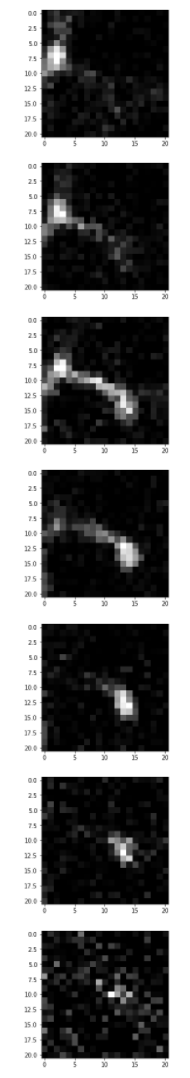
\includegraphics[width=0.2\linewidth]{neuron-slices}

\section{Foreground Analysis}
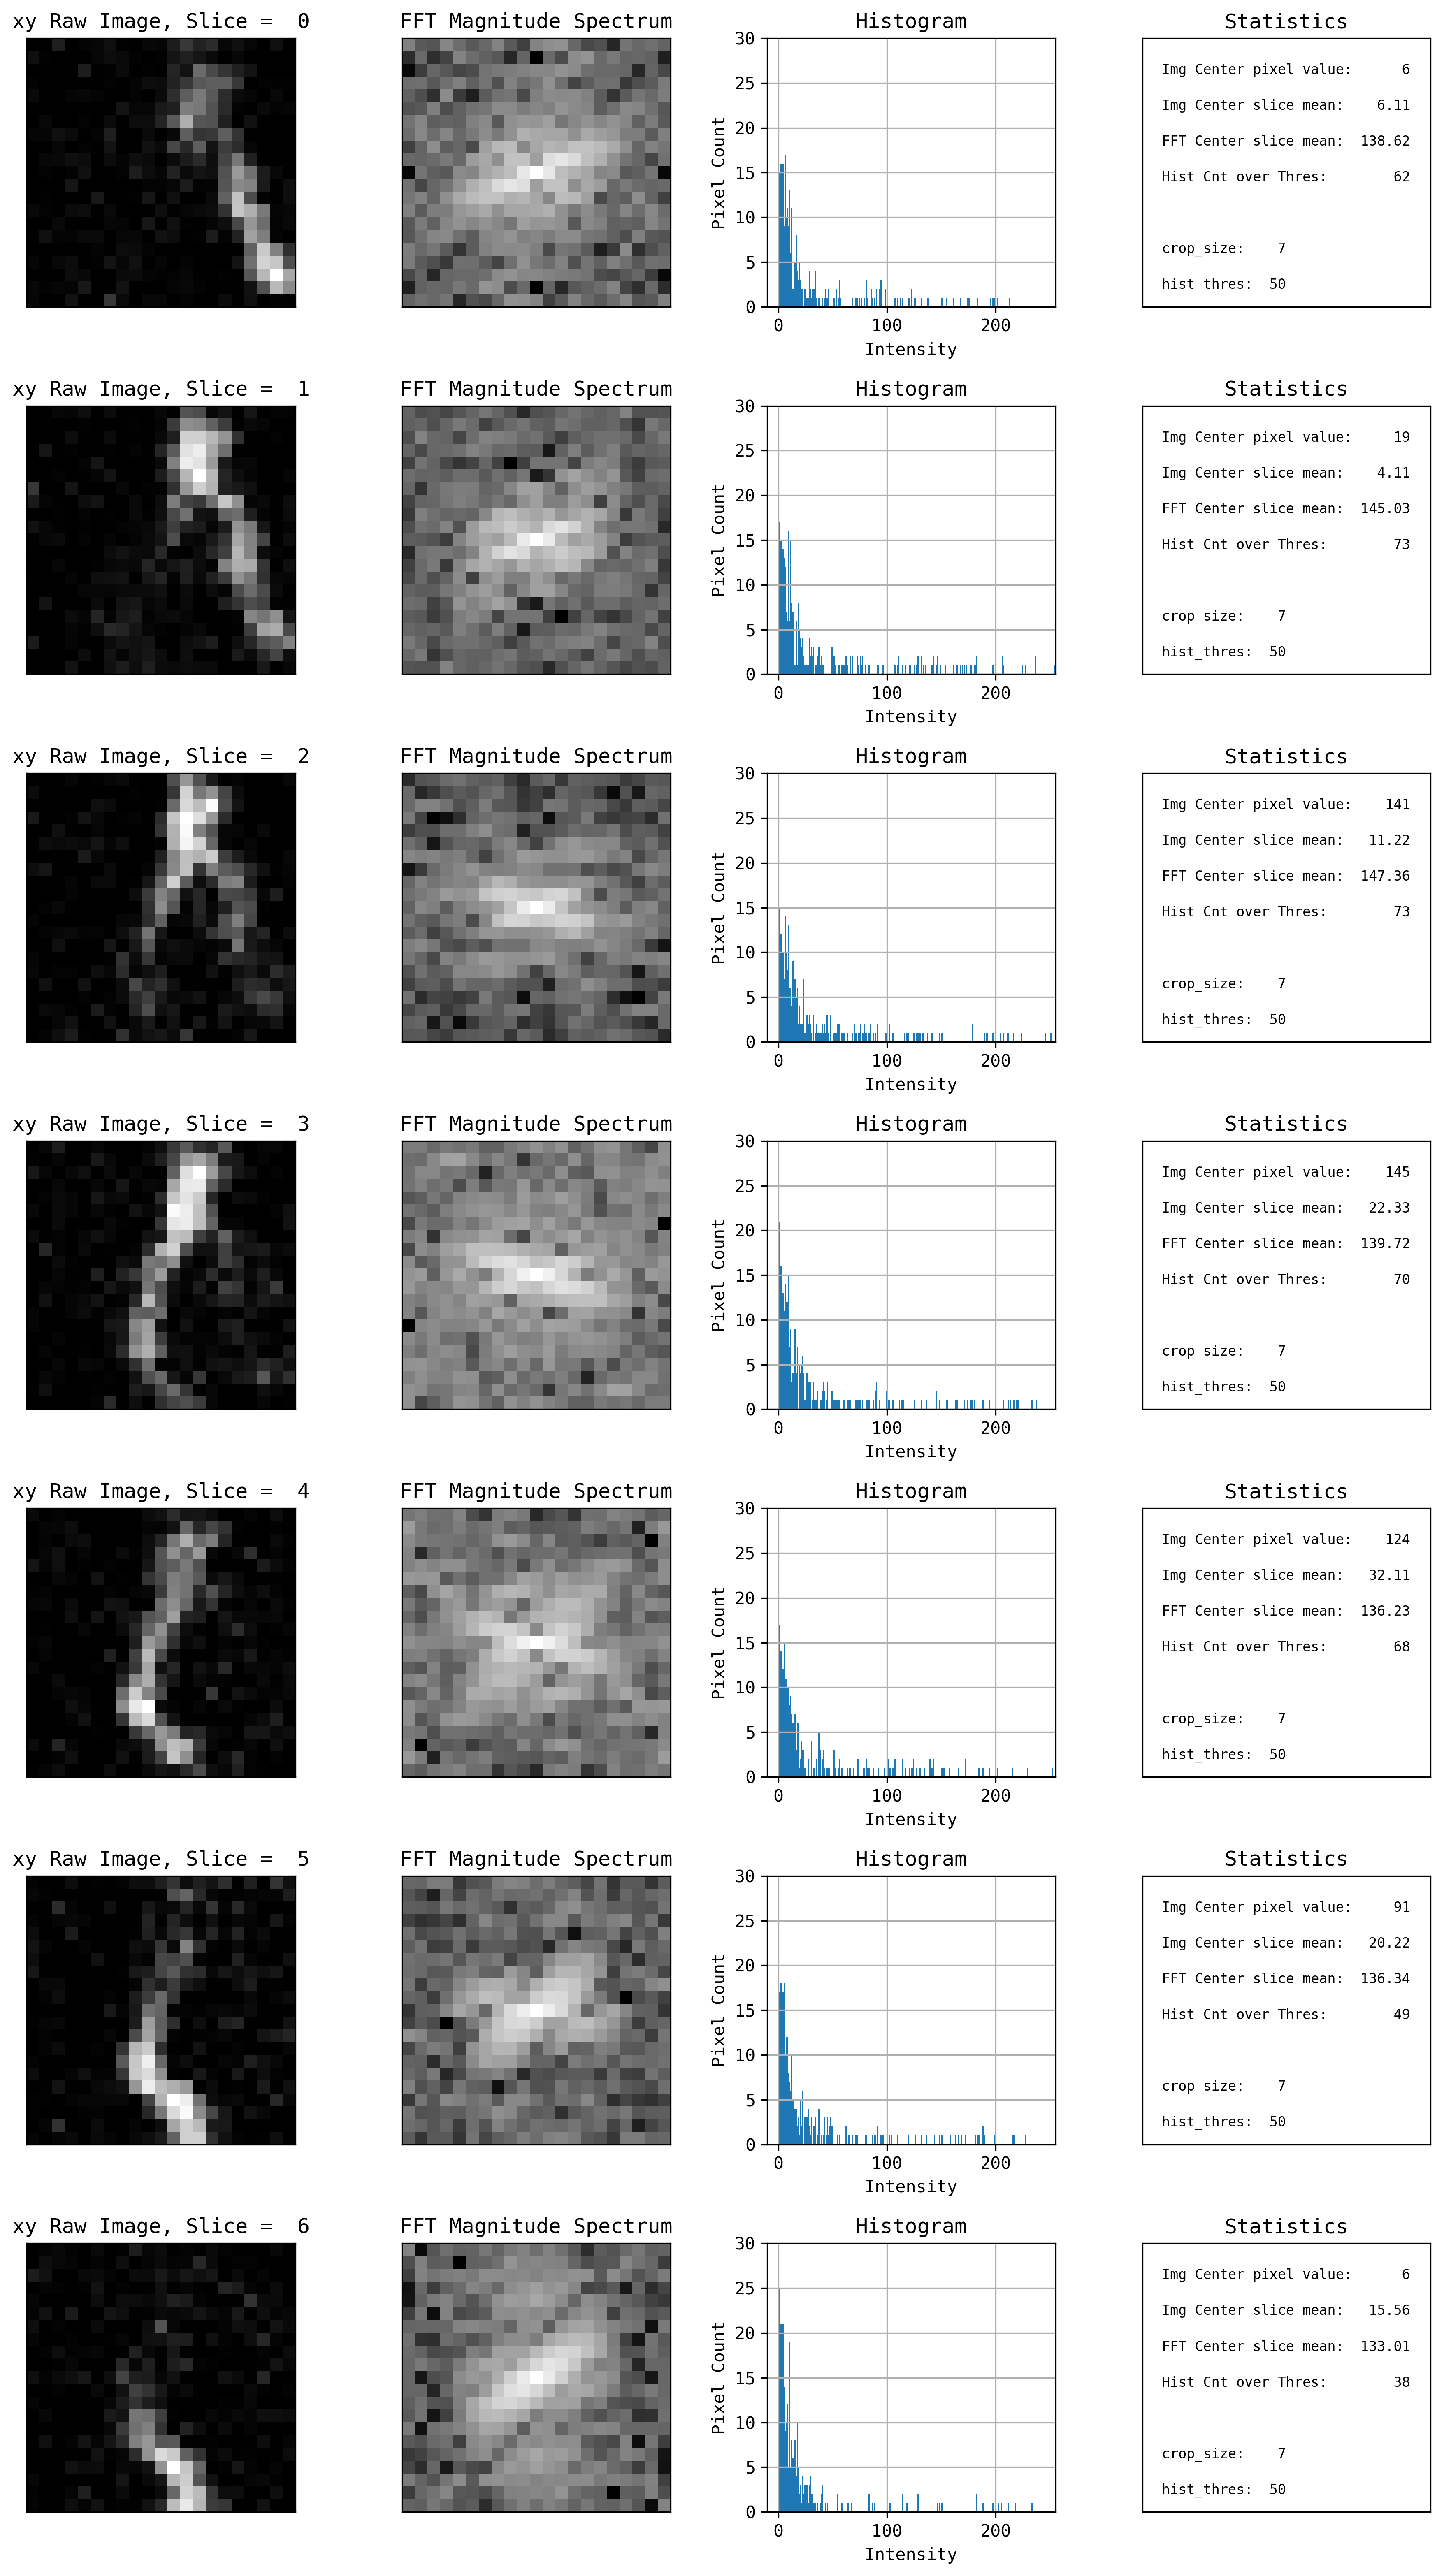
\includegraphics[width=0.7\linewidth]{foreground-xy-1}

\section{Background Analysis}
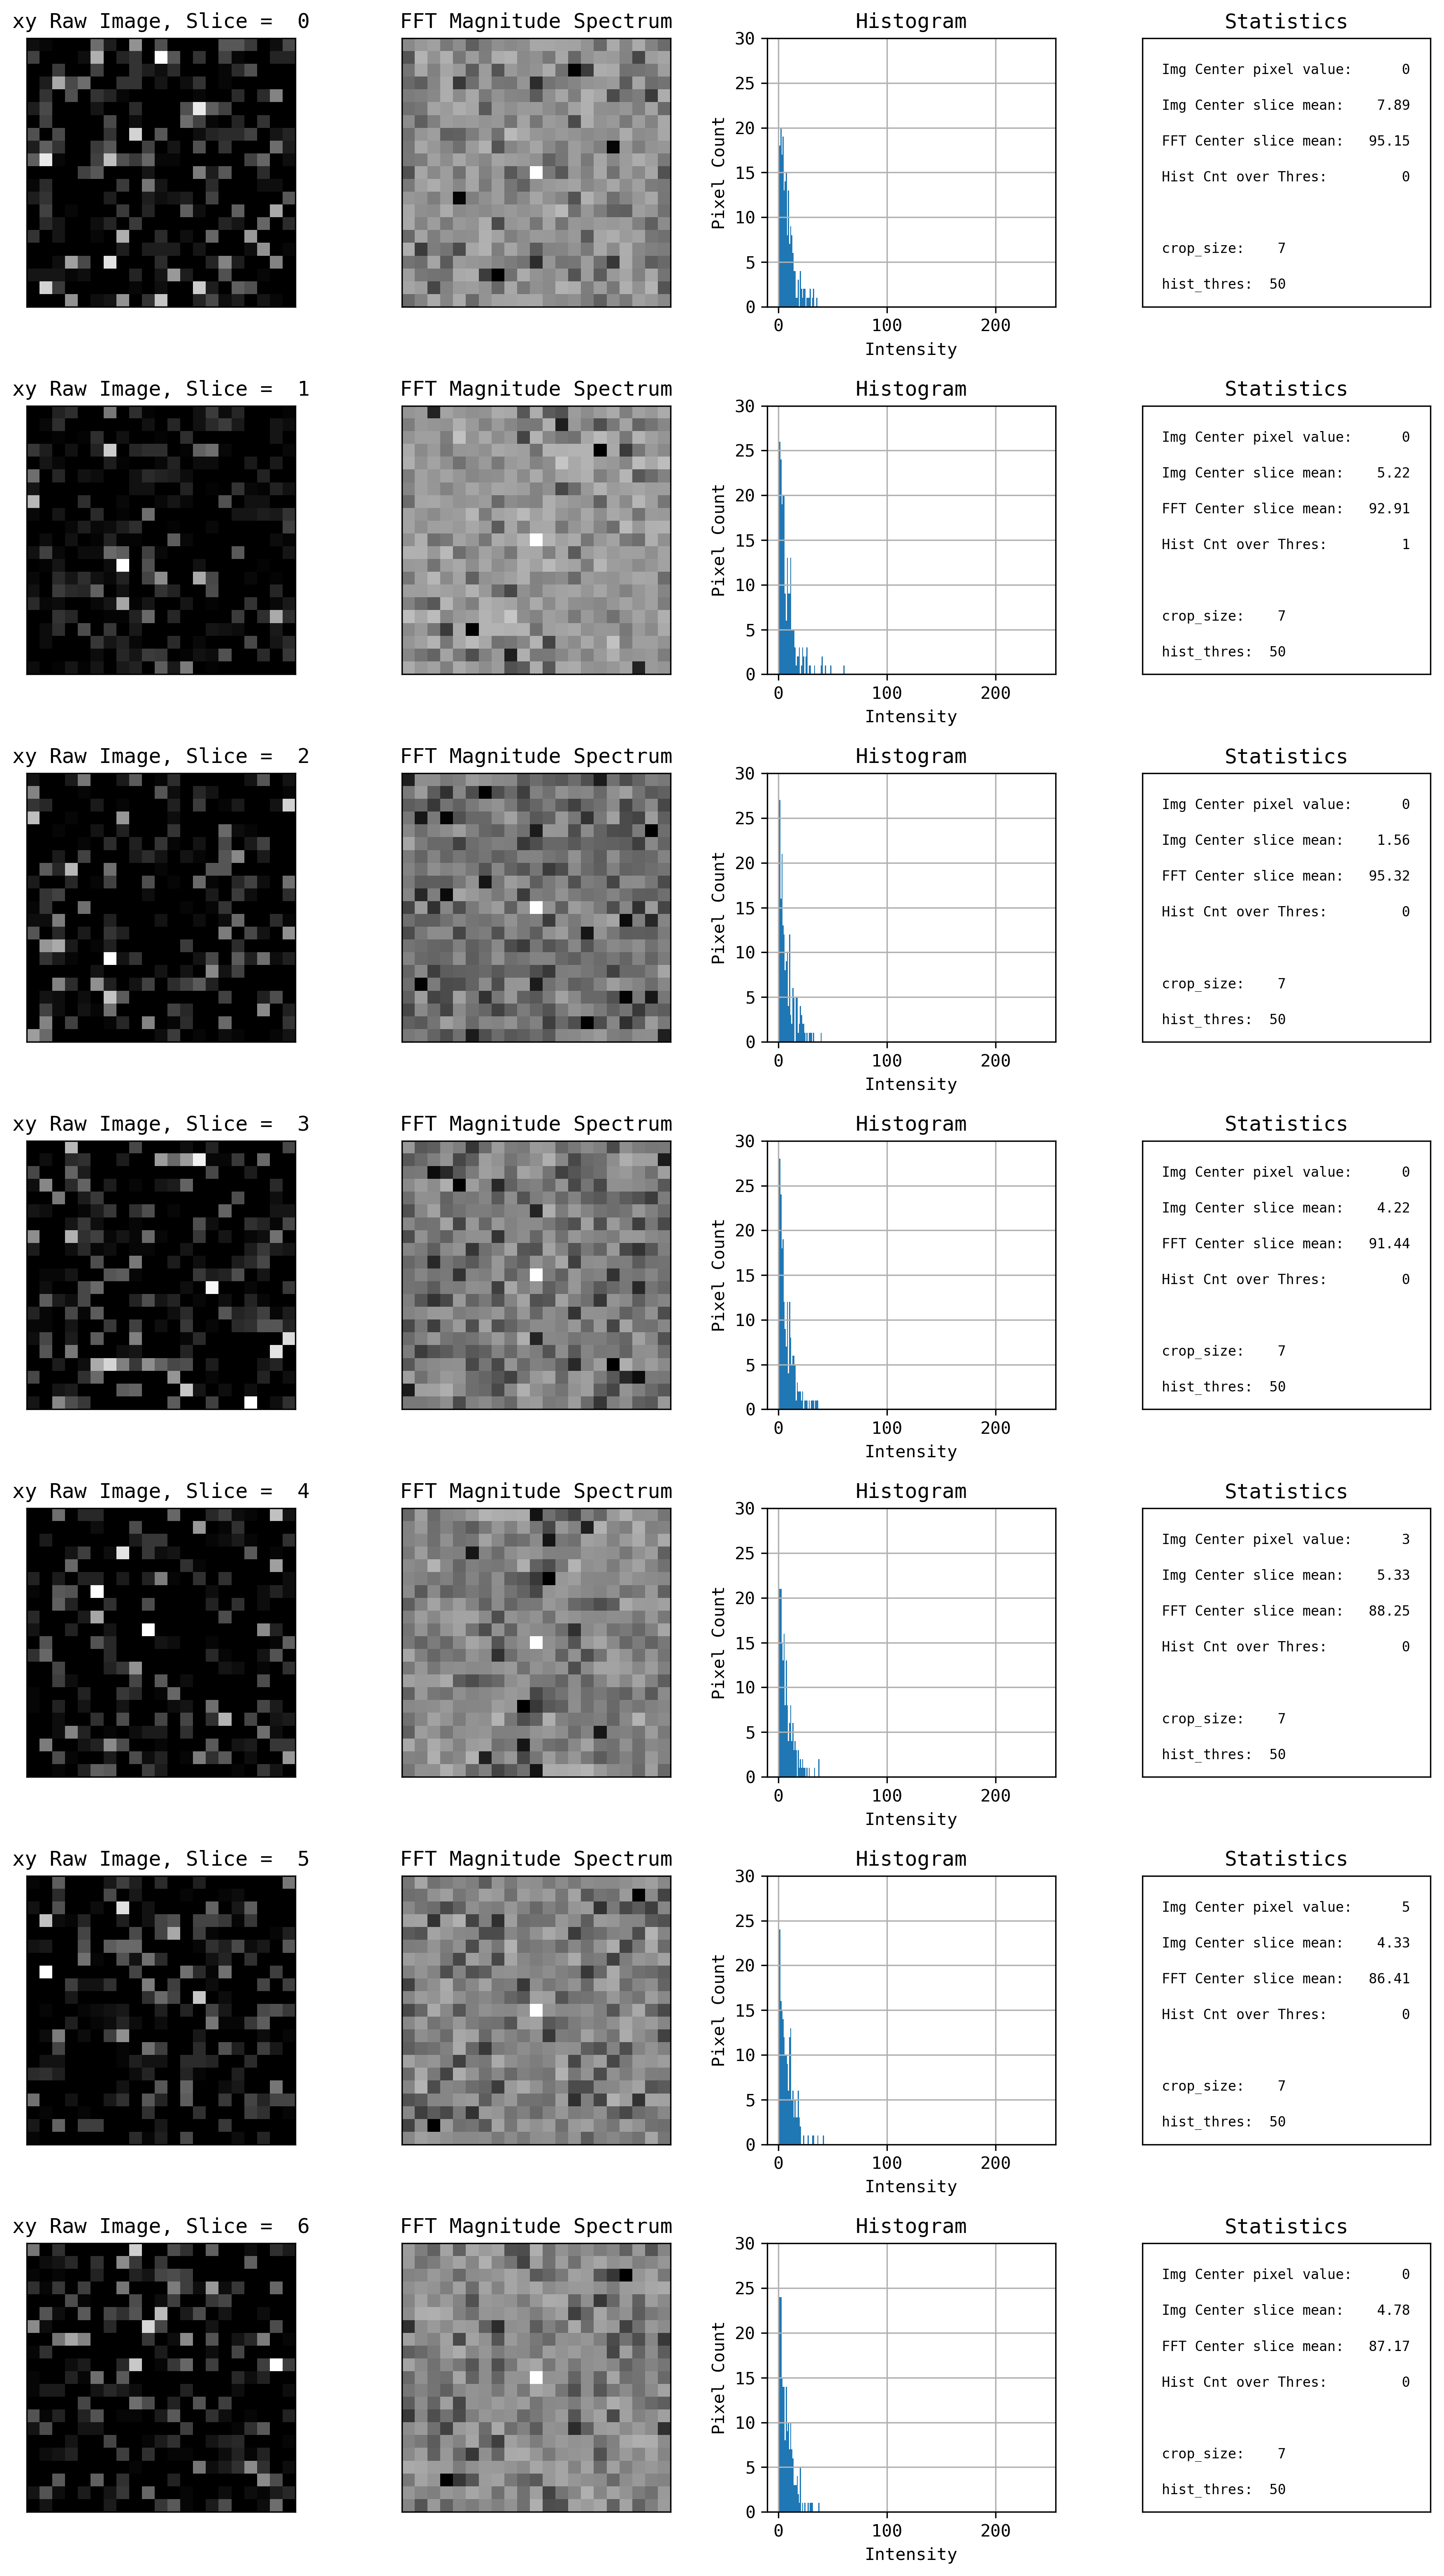
\includegraphics[width=0.7\linewidth]{background-xy-0}

\section{Classification Comparison Test}
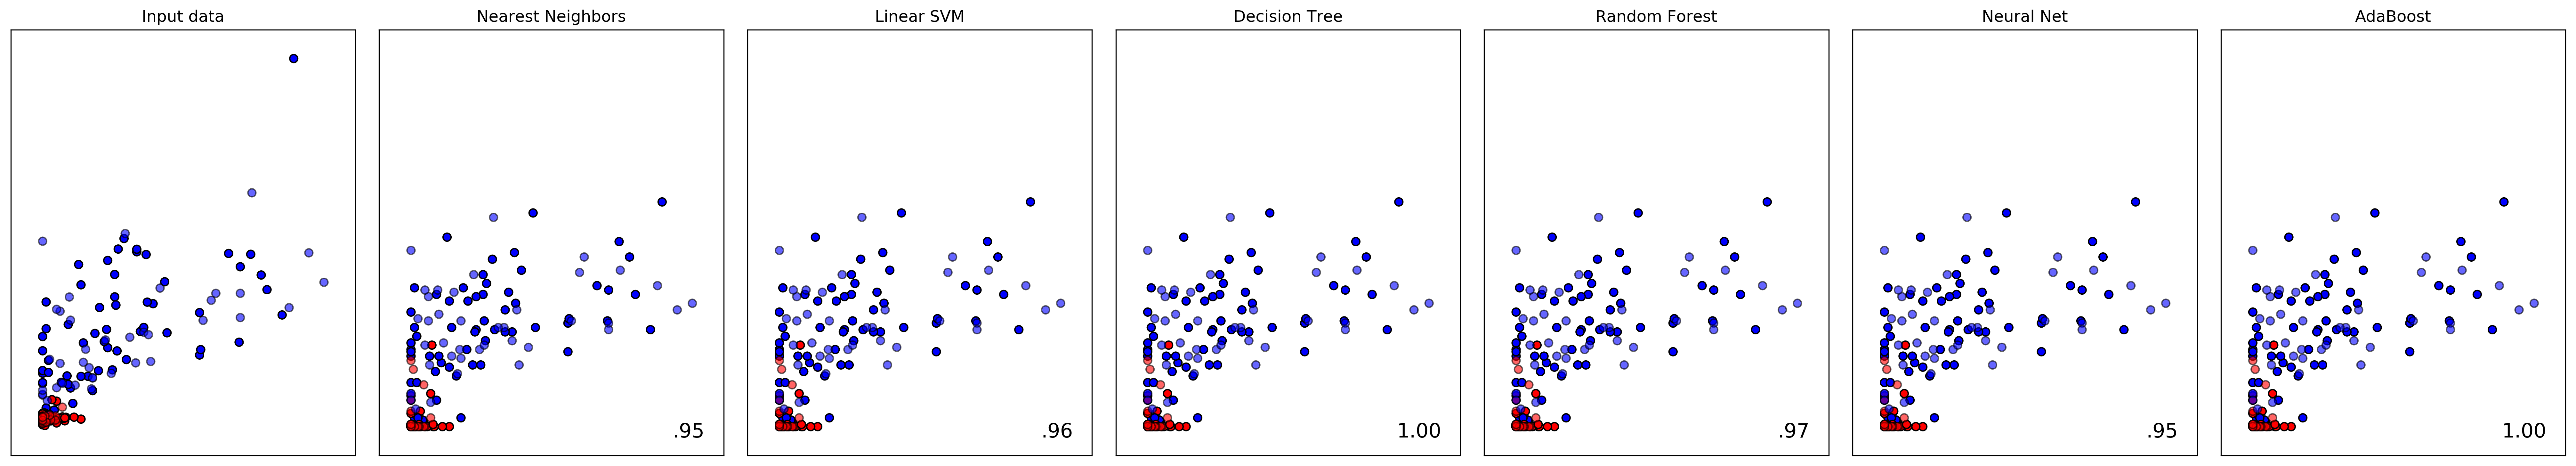
\includegraphics[width=0.7\linewidth]{classification-test}



\end{document}
